\section*{Appendix A - Function for Primary Section}\label{subsection:primary_calcs}

\begin{minted}[frame=lines,fontsize=\footnotesize,linenos, baselinestretch=1.0]{python}

def primary(save_flag:bool):

    DENSITY_AIR, DENSITY_FUEL, MW_AIR, MW_FUEL = thermo.calc_AirProperties()
    AFR_STOIC = thermo.calc_AirFuelRatio(MW_AIR, MW_FUEL, stoic=True)

    # Design variables
    iters = 51
    V_FUEL_RANGE    =   np.linspace(60, 110, iters)
    V_AIR_RANGE     =   np.linspace(40, 90, iters)

    data_store = []

    for V_FUEL, V_AIR in itertools.product(V_FUEL_RANGE, V_AIR_RANGE):

        mf_fuel         =   DENSITY_FUEL * A_FUEL * V_FUEL
        mf_air_primary  =   DENSITY_AIR  * A_AIR  * V_AIR

        afr_rich        =   mf_air_primary / mf_fuel
        eqr_rich        =   AFR_STOIC / afr_rich

        # Calculate the momentum flux
        momentum_flux = (DENSITY_FUEL * (V_FUEL)**2) / (DENSITY_AIR * V_AIR ** 2)

        data_store.append({
            'EQR_RICH'          :       eqr_rich,
            'AFR_RICH'          :       afr_rich,
            'V_FUEL'            :       V_FUEL,
            'MASSFLOW_FUEL'     :       mf_fuel,
            'V_AIR'             :       V_AIR,
            'MASSFLOW_AIR_P'    :       mf_air_primary,
            'J'                 :       momentum_flux,
        })

    df = pd.DataFrame(data_store)
    print(df)

    df = df[(df['EQR_RICH'] >= 1.24) & (df['EQR_RICH'] < 1.25)]
    df = df[(df['J'] > 2) & (df['J'] < 3)]


    print(df)

    if save_flag:
        df_out = df.round(6)
        ut.make_dir(DATA_DIR)
        df_out.to_csv(os.path.join(DATA_DIR, 'd_points.csv'), index=False)

    if '--plot' in sys.argv:
        
        g = sns.relplot(
            data=df,
            x="EQR_RICH", y="J", col="V_FUEL", hue="V_AIR",
            kind="scatter", palette=palette, col_wrap=3,
            height=4, aspect=.75, facet_kws=dict(sharex=False),
        )

        ut.make_dir(FIG_DIR)

        plt.savefig(FIG_DIR + '/plt_comp.png', format='png')
        plt.savefig(FIG_DIR + '/plt_comp.eps', format='eps')
    
    return AFR_STOIC
\end{minted}

\clearpage

\section*{Appendix B - Function for Secondary Section}

\begin{minted}[frame=lines,fontsize=\footnotesize,linenos, baselinestretch=1.0]{python}
def secondary(silent:bool=True) -> float:

    """
    For the secondary part, the target is to have an equivalence ratio of 0.42.
    How do we get that? Interesting.
    
    """

    DENSITY_AIR, DENSITY_FUEL, MW_AIR, MW_FUEL = thermo.calc_AirProperties()
    AFR_STOIC = thermo.calc_AirFuelRatio(MW_AIR, MW_FUEL, stoic=True)

    # Following is the desgin point selected from the primary calculations.
    EQR_GLOBAL:float = 0.42
    PRIMARY_VARS:dict = {
        'EQR_RICH': 1.245,
        'AFR_RICH': 4.854891, 
        'V_FUEL': 99.0, 
        'MASSFLOW_FUEL': 0.007339, 
        'V_AIR': 65.0, 
        'MASSFLOW_AIR_P': 0.035631, 
        'J': 2.738813
        }

    MASSFLOW_AIR_P = PRIMARY_VARS['MASSFLOW_AIR_P']
    AFR_GLOBAL = AFR_STOIC / EQR_GLOBAL
    MASSFLOW_AIR_GLOBAL = PRIMARY_VARS['MASSFLOW_FUEL'] * AFR_GLOBAL

    MASSFLOW_AIR_S = MASSFLOW_AIR_GLOBAL - MASSFLOW_AIR_P

    if silent:
        print(MASSFLOW_AIR_S)
        return MASSFLOW_AIR_S
    else:
        print("")
        print('Combustor mass flows:')
        print(f"{'Quantity':<20} {'Value':>15} {'Unit':<10}")
        print("-" * 50)
        print(f"{'Global mass flow':<20} {MASSFLOW_AIR_GLOBAL:>15.6f} {'kg/m3':<10}")
        print(f"{'Primary mass flow':<20} {PRIMARY_VARS['MASSFLOW_AIR_P']:>15.6f} {'kg/m3':<10}")
        print(f"{'Secondary mass flow':<20} {MASSFLOW_AIR_S:>15.6f} {'kg/m3':<10}")

\end{minted}

\clearpage


\section*{Appendix B - Functions for RQL reactor in Cantera}


\textbf{RICH ZONE}

\begin{minted}[frame=lines,fontsize=\footnotesize,linenos, baselinestretch=1.0]{python}
def rich(
    eqr: float, mixture:ct.composite.Solution
) -> tuple:
    """
    Function for calculating the reaction characteristics in the rich burn zone.
   
    Inputs:
    ------
    - eqr_rich: equivalence ratio for the rich zone
    - air: cantera air
    - fuel: cantera fuel
    - mixture: init mixture gas
   
    Returns:
    -------
    - flame: solved FreeFlame object
    - gas_mix: cantera Solution object with the mixed state
    - outlet_state: string of species mass fractions at the outlet
    """

    # Solve flame simulation
    initial_grid = np.linspace(0, 0.059917, 101)
    flame = ct.FreeFlame(mixture, initial_grid)
    flame.energy_enabled = True
    flame.set_refine_criteria(ratio=3, slope=0.2, curve=0.2)
    
    try:
        flame.solve(loglevel=1, refine_grid=True, auto=False)
        solution_successful = True
    except:
        flame.set_refine_criteria(ratio=3, slope=0.1, curve=0.1)
        try:
            flame.solve(loglevel=1, refine_grid=True, auto=True)
            solution_successful = True
        except:
            solution_successful = False
    
    if solution_successful:
        print(f'Phi={eqr}: Outlet temperature = {flame.T[-1]:.1f} K')
        try:
            no_index = mixture.species_index('NO')
            print(f'NOx at outlet: {1000000*flame.Y[no_index][-1]:.2f} ppm')
        except ValueError:
            print("NO species not found in mechanism")

        outlet_state = ''
        #print("\n\n")
        #print(f"{'Species':<20} {'Mass Fraction':>15}")
        #print("-" * 50)
        for i in range(0, mixture.n_species):
            species_name = mixture.species_name(i)
            species_mass_fraction = flame.Y[mixture.species_index(species_name)][-1]
            if i == 0:
                outlet_state += f'{species_name}:{species_mass_fraction:.9f}'
            else:
                outlet_state += f',{species_name}:{species_mass_fraction:.9f}'
            #print(f"{species_name:<20} {species_mass_fraction:>15.9f}")
        #print("\n\n")

        return flame, mixture, outlet_state
    
    else:
        print("Flame solution failed. Returning None.")
        return None, mixture, None

\end{minted}

\clearpage


\textbf{MIXING ZONE}

\begin{minted}[frame=lines,fontsize=\footnotesize,linenos, baselinestretch=1.0]{python}
def mixing(
    gas_a:ct.composite.Solution, gas_b:ct.composite.Solution, mdot_a:float, mdot_b:float
) -> tuple:
    """
    Description:
    -----------
    This function mixes two gases.
    https://cantera.org/3.1/examples/python/reactors/mix1.html#sphx-glr-examples-python-reactors-mix1-py

    Inputs:
    ------
    gas_a: This is the combustion gas obtained from the first part of the reaction.
    gas_b: This is the quench air obtained from the HPC.
    EQR  : The equivalence ratio of the mixture.

    Returns:
    ------
    boundary species for lean burn
    
    """

    # Create reservoirs for storing mixture data.
    reservoir_a = ct.Reservoir(gas_a, name='gas a res')
    reservoir_b = ct.Reservoir(gas_b, name='gas b res')
    downstream  = ct.Reservoir(gas_b, name='outlet reservoir')

    # Create a reactor for the mixer. A reactor is required instead of a reservoir, 
    # since the state will change with time if the inlet mass flow rates change or if there 
    # is chemistry occurring. FROM CANTERA DOCUMENTATION
    mixer = ct.IdealGasReactor(gas_a, name='Mixer')

    # Create the mass flow controllers.
    mfc1 = ct.MassFlowController(reservoir_a, mixer, mdot=mdot_a, name="gas_a")
    mfc2 = ct.MassFlowController(reservoir_b, mixer, mdot=mdot_b, name="gas_b")


    outlet = ct.Valve(mixer, downstream, K=10.0, name="Valve")
    sim = ct.ReactorNet([mixer])

    sim.advance_to_steady_state()
    print(mixer.thermo.report())

    # Prepare the species from this reactor to the one with Lean burner calculation
    boundary_species:str = ''
    for i in range(100000):
        try:
            name = mixer.thermo.species_name(i)
            y_val = mixer.thermo.Y[mixer.thermo.species_index(name)]
            if i == 0:
                boundary_species += '%s:%.8f'%(name,y_val)
            else:
                boundary_species += ' ,%s:%.8f'%(name,y_val)
        except:
            break
   
    return mixer, boundary_species
\end{minted}

\clearpage

\textbf{LEAN ZONE}

\begin{minted}[frame=lines,fontsize=\footnotesize,linenos, baselinestretch=1.0]{python}
def lean(
    gas:ct.composite.Solution, mdot:float, geom:dict
) -> None:
    print("Computing LEAN zone.")

    n_steps = 2000
    dz = geom['length'] / n_steps
    r_vol = geom['area'] * dz

    # Make a new reactor for lean burn
    lean_reactor = ct.IdealGasReactor(gas)
    lean_reactor.volume = r_vol
    upstream = ct.Reservoir(gas, name='upstream')
    downstream = ct.Reservoir(gas, name='downstream')
    m = ct.MassFlowController(upstream, lean_reactor, mdot=mdot)
    v = ct.PressureController(lean_reactor, downstream, primary=m, K=1e-5)
    sim2 = ct.ReactorNet([lean_reactor])

    # define time, space, and other information vectors
    z2 = (np.arange(n_steps) + 1) * dz
    t_r2 = np.zeros_like(z2)  # residence time in each reactor
    u2 = np.zeros_like(z2)
    t2 = np.zeros_like(z2)
    states2 = ct.SolutionArray(lean_reactor.thermo)

    # iterate through the PFR cells
    for n in range(n_steps):
        # Set the state of the reservoir to match that of the previous reactor
        gas.TDY = lean_reactor.thermo.TDY
        upstream.syncState()
        # integrate the reactor forward in time until steady state is reached
        sim2.reinitialize()
        sim2.advance_to_steady_state()
        # compute velocity and transform into time
        u2[n] = mdot / geom['area'] / lean_reactor.thermo.density
        t_r2[n] = lean_reactor.mass / mdot  # residence time in this reactor
        t2[n] = sum(t_r2)
        # write output data
        states2.append(lean_reactor.thermo.state)

    print('Final Temperature is ',states2.T,'K')
    print(f"NOx is {1000000*states2.Y[-1, gas.species_index('NO')]} ppm")

    return gas
\end{minted}


\clearpage


\textbf{RQL Function}

\begin{minted}[frame=lines,fontsize=\footnotesize,linenos, baselinestretch=1.0]{python}
def RQL(
    eqr_rich:float, eqr_lean:float
) -> None:
    """
    NOTE:
    This function should have 3 parts:
    1. Rich burn reaction.
    2. Mixing of the secondary air.
    3. Lean burn reaction.

    And also two misc steps:
    1. Before the program runs, need to generate directories.
    """
    print("Initializing the RQL reaction mechanism.")

    # TODO Perform the preprocessing step:
    # Create temp directories for storing data between separate RQL stages.
    # INIT gases

    PFR:dict = {
        'length': 0.5,     # [m]
        'radius': 0.018823,     # [m]
        'area'  : 1.e-3,     # [m^2]
        'volume': 0.000048,     # [m^3]
        'vel'   : 20            # [m/s] 
    }

    fuel        = ct.Solution(SanDiegoMech)
    fuel.TPX    = T_FUEL, P_FUEL, {'NH3': 1.0}

    air         = ct.Solution(SanDiegoMech)
    air.TPX     = T_AIR, P_AIR, {'O2': 1.0, 'N2': 3.76}

    rich_gas_thermo, inlet_bounbdary_species = rt.mixing(gas_a=fuel, gas_b=air, mdot_a=0.007339, mdot_b=0.035631)
    
    # Create the rich burn gas
    rich_gas = ct.Solution(SanDiegoMech)    
    rich_gas.TPY = rich_gas_thermo.thermo.T, rich_gas_thermo.thermo.P, rich_gas_thermo.thermo.Y
    rich_flame, rich_out, rich_outlet_state = rt.rich(eqr=1.24, mixture=rich_gas)
    print(rich_out.report())

    air_secondary         = ct.Solution(SanDiegoMech)
    air_secondary.TPX     = T_AIR, P_AIR, {'O2': 3.0, 'N2': 3*3.76}

    # Mix the output of rich flame with secondary air.
    lean_gas_thermo, lean_inlet_boundary_species = rt.mixing(gas_a=rich_out, gas_b=air_secondary, mdot_a=0.007339+0.035631, mdot_b=secondary())
    
    # Create the lean burn gas
    lean_gas = ct.Solution(SanDiegoMech)
    lean_gas.TPY = lean_gas_thermo.thermo.T, lean_gas_thermo.thermo.P, lean_gas_thermo.thermo.Y
    print(lean_gas.report())
\end{minted}

\clearpage

\section*{Appendix D - RQL Combustor Drawing} \label{subsection:rql_dim_drawing}


\begin{figure}[H]
    \centering
    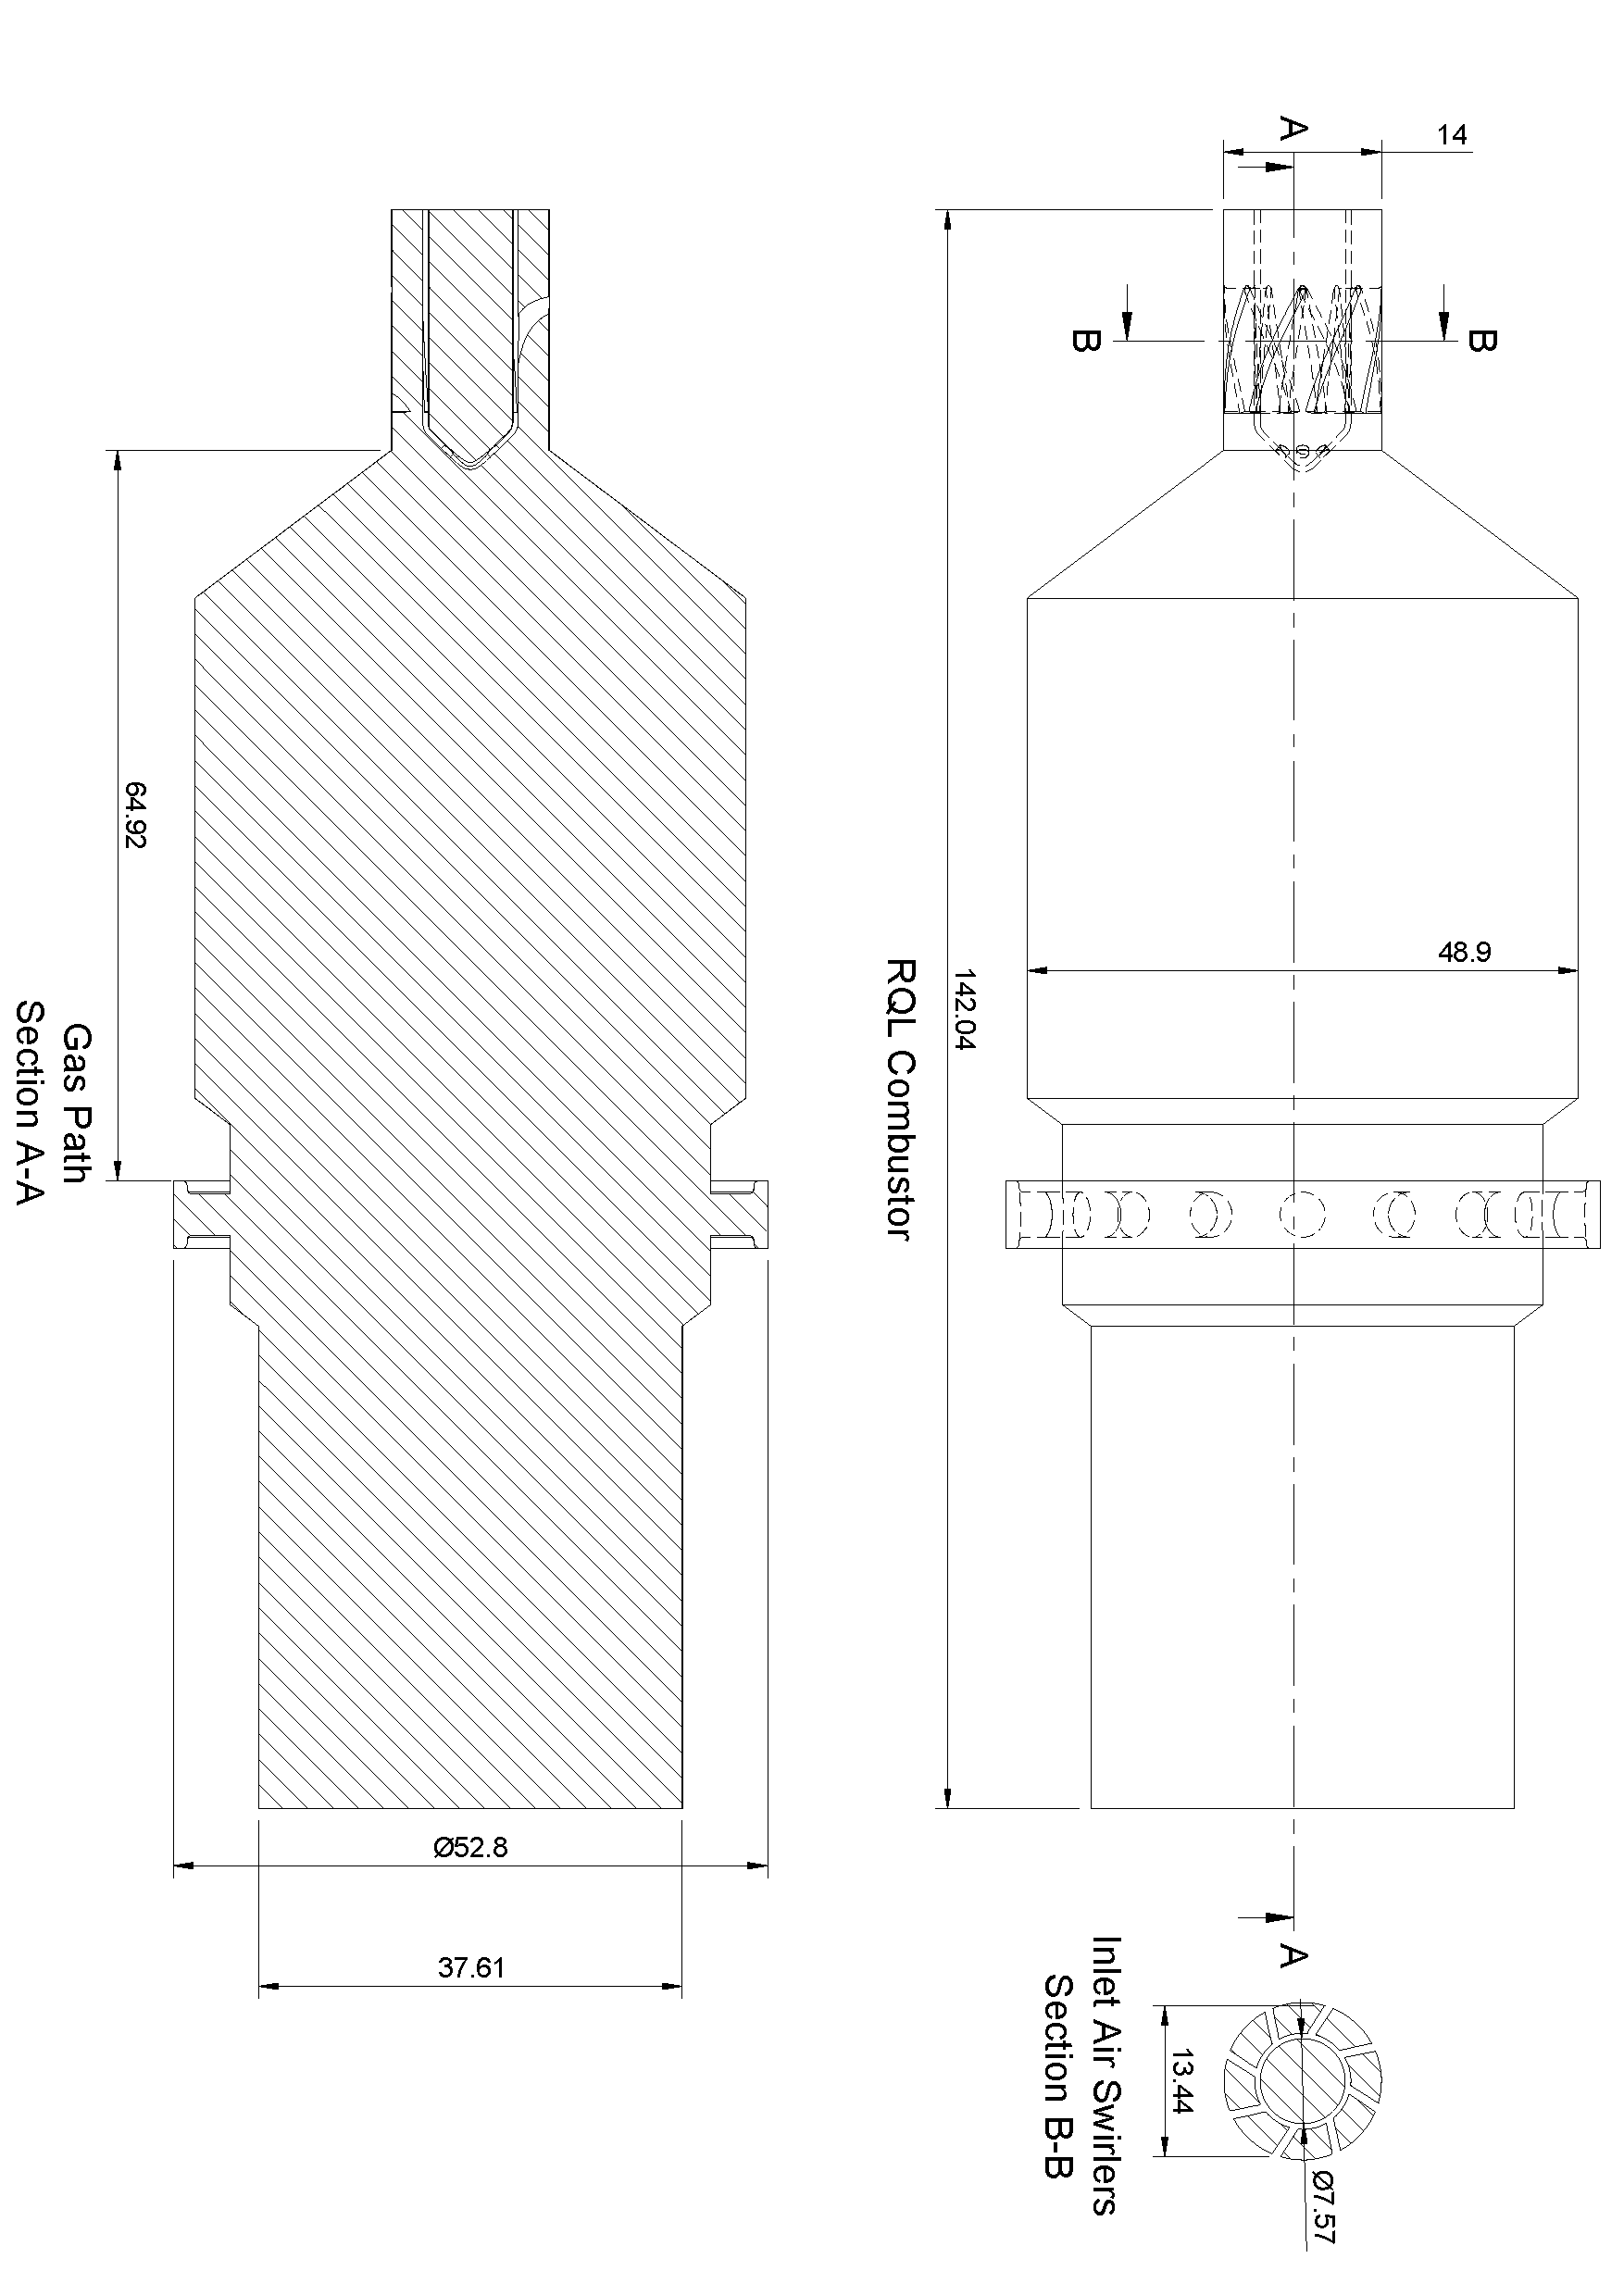
\includegraphics[width=0.9\linewidth]{figs/RQL Combustor DWG.pdf}
    \caption{Drawing for the RQL combustor.}
    \label{fig:Drawing_RQL}
\end{figure}
